\documentclass[12pt]{article}
\usepackage[a4paper, portrait, margin=1cm, right=1cm]{geometry}
\usepackage{fontspec}
\usepackage[fleqn]{amsmath}
\usepackage{setspace}
\usepackage{graphicx}
\usepackage{multirow}

\graphicspath{./graphics/}
\setmainfont[Ligatures=TeX]{Linux Libertine}

\title{Информационные технологии. Лекция 05. Вопросы воздействия окружающей среды}
\author{Студент группы 2305 Макурин Александр}
\date{27 марта 2023}

\begin{document}

\maketitle
\begin{sloppypar}
    $Environment = Env \cup E$

    Окружающая среда — те факторы, которые влияют на систему.

    $E = \bigcup S^i_j$

    $S_E = f(Env, E)$, где $S_E$ — состояние системы, $Env$ — окружающая среда, воздействующая на систему, $E$ — остальная окружающая среда.

    Пусть существуют факторы $x_i^t$, являющиеся частями окружающей среды: $\exists x_i^t : x_i^t \in E$.

    Эти факторы делятся на значимые и незначимые:
    \begin{itemize}
        \item Значимые $x_i$: $\Delta S \not\approx 0$ при изменении фактора: $x_i^{t + 1} \neq x_i^t$.
        \item Незначимые $x_i$: $\Delta S \approx 0$ при изменении фактора: $x_i^{t + 1} \neq x_i^t$.
    \end{itemize}

    $E = X_{\text{зн}} \cup X_{\text{незн}}$, где $E$ — вся окружающая среда, $X_{\text{зн}}$ — значимые факторы, $X_{\text{незн}}$ — незначимые факторы.

    $Env = \bigcup X_{\text{зн}}$ — окружающая среда, воздействующая на систему, есть совокупность значимых факторов.

    $S_E^t = f(E^t, X^t, \{S_E^{t-1}\})$ — состояние системы.

    \section{Три основных свойства системы}
    $e_i \in E$, $e_i$ — элемент системы, $E$ — система.

    $P_{e_i}$ — свойства элемента $e_i$.

    $P_{e_i} = \{P_{comm}, P_{act}, P_{analysis}\}$

    $P_{comm}$ — способность элемента к коммуникации (e.g. передатчик)

    $P_{act}$ — способность элемента к воздействию на окружающую среду (e.g. манипулятор)

    $P_{analysis}$ — способность элемента к анализу (e.g. микроконтроллер)

    $P^*_{...}$ — свойство находится в идеальном состоянии.

    Если $P_{e_i} = \{P^*_{comm}, P^*_{act}, P^*_{analysis}\}$, то свойства элемента $e_i$ находятся в идеальном состоянии.

    Если существуют значимые факторы, такие что $P_{e_i}^t \rightarrow 0$, то среда очень агрессивна.

    $S_E^t = f(E^t, \{S_E^{t-1}\})$ — состояние системы в идеальной среде. Тогда $S_E^t$ зависит только от прежнего состояния системы.

    $S_E^t = f(E^t, X^{Env}, \{S_E^{t-1}\})$ — состояние системы в агрессивной среде.

    Обозначим за $\alpha = \dfrac{\delta^2S}{\delta^2t}$ и $\overline{\alpha} = \dfrac{\delta^2S}{\delta^2t}$ скорости деградации системы в идеальных условиях и с учётом окружающей среды соответственно. Тогда:
    \[ |a| << |\overline{a}| \]

    $G$ — цель системы. $G = \{g(TK)\}$, $TK$ — задачи, $g$ — функция выполнения задачи.

    $g(TK^i) = <f(Env), f(E, X^{Env}, \{S^{t - 1}\})> = <S_{env}^t, S_E^t>$

    Мы хотим, чтобы $G \rightarrow max$, следовательно $g \rightarrow max$, следовательно, т. к. $f(Env) = const$, $f(E, X^{Env}, \{S^{t - 1}\}) \rightarrow max$.

    
\includegraphics[width=0.5\textwidth]{graphics/деградация.png}

    Ложно агрессивная среда — реальное изменение состояния системы стремится к нулю, а изменение рабочего состояния системы к нулю не стремится: $\Delta S_E^{fact} \rightarrow 0,\ \Delta S_E^w \not \rightarrow 0$

    Влияние окружающей среды состоит из двух частей — функции оценки и реального состояния: $f(out(X^{env}))$, где $out$ — функция оценки, а $X^{env}$ — реальное состояние.

    В идеальном случае: $out(X^{env}) \rightarrow X^{env}$. В реальности $P(out(X) = X) < 1$ всегда.

    \section{Основные проблемы функционирования}
    \begin{enumerate}
        \item Шум: $E(out(X_i, n)) = X^{env} + \overline{n}$. Здесь $x_i$ — шум от окружающей среды, $n$ — шум от аппаратной части, $\overline{n}$ — шум.
        \item Сбои: $E(out) \neq X^{env} (+ \overline{n})$ — нельзя оценить какой будет шум.
    \end{enumerate}

    \section{Задачи}

    Функции обработки факторов внешней среды:
    \begin{enumerate}
        \item $c: out(c(X^{env})) \rightarrow X^{env}$ — возможно, фильтр. Применяется к внешней среде прежде, чем её оценивать
        \item $d : d(out(X^{env}))$ — возможно, статистический анализ. Применяется для корректировки результатов функции оценки.
        \item $fa : f(fa(out(X^{env}))) \rightarrow max$ — СППР
    \end{enumerate}

    СППР — система поддержки принятия решений.

    Первые две задачи могут быть решены посредством машинного обучения.

    Если скомпоновать все функции вместе, то получится:
    \[ f(fa(d(out(c(X^{env}))))) \]

    \section{Человек}

    $H = user \ \cup \ component \ \cup \ env$. $H$ — люди, $user$ — пользователи системы, $component$ — люди-компоненты системы, $env$ — люди как окружающая среда. $env$ отдельно не рассматривается, т. к. ничем не отличается от обычной окружающей среды.

    $user : R = P \cdot V$, где $R$ — риск, $P$ — вероятность проблемы, $V$ — ущерб.

    Ущерб делится на:
    \begin{enumerate}
        \item Ущерб состоянию человека (здоровью)
        \item Материальный ущерб
        \item Недостигнутые цели
    \end{enumerate}

    $\begin{cases}
            G \rightarrow max \\
            R \rightarrow min
        \end{cases}\Rightarrow
        \begin{cases}
            G \rightarrow max                                                             \\
            \text{Hu} \rightarrow \text{Hu}^0 \text{ — сохранение состояния пользователя} \\
            E \rightarrow E^0 + \nu \text{ — сохранение системы, где $\nu$ — дополнительные потери}
        \end{cases}
    $

    $\Rightarrow \begin{cases}
            G \rightarrow max                                                    \\
            \text{Hu} \rightarrow \text{Hu}^0 \text{ — сохранение пользователей} \\
            H_{env} \rightarrow H_{env}^0 \text{ — сохранение окружающих людей}  \\
            P_E^t \rightarrow P_E^0 + \nu \text{ — сохранение свойств системы}
        \end{cases}$

    \section{Производство}


    \subsection{Жизненный цикл. Основные этапы}
    \begin{tabular}{|c|l|c|}
        \hline
        № & Этап (для программной состовляющей)                              & Средние затраты (в \%) \\
        \hline
        1 & Анализ требований (составление ТЗ, определение основных функций) & 3                      \\
        \hline
        2 & Проектирование и разработка спецификаций                         & 8                      \\
        \hline
        3 & Кодирование                                                      & 7                      \\
        \hline
        4 & Тестирование                                                     & 15                     \\
        \hline
        5 & Релиз (выпуск завершенной версии и ввод в эксплуатацию)          & \multirow{2}{*}{67}    \\
        \cline{1-2}
        6 & Сопровождение                                                    &                        \\
        \hline
    \end{tabular}

    \subsection{ГОСТ 34.601-90. Автоматизированные системы. Стадии создания}

    \begin{itemize}
        \item Формирование требований
              \begin{itemize}
                  \item Обследование объекта и обоснование необходимости создания
                        \begin{itemize}
                            \item Сбор данных об объекте
                            \item Оценка качества функционирования, выявление проблем
                            \item Оценка целесообразности
                        \end{itemize}
                  \item Формирование требований пользователей
                        \begin{itemize}
                            \item Исходные данные для требований
                            \item Формулировка и оформление требований
                        \end{itemize}
              \end{itemize}
        \item Разработка концепции
              \begin{itemize}
                  \item Изучение объекта
                  \item Проведение НИР (научно-исследовательских работ)
                  \item Разработка вариантов концепции
                        \begin{itemize}
                            \item Альтернативные варианты концепций
                            \item Необходимые ресурсы
                            \item Преимущества и недостатки
                            \item Определение условий приемки
                            \item Оценка эффектов от системы
                        \end{itemize}
              \end{itemize}
        \item Техническое задание — разработка, оформление, согласование и утверждение ТЗ
        \item Эскизный проект
              \begin{itemize}
                  \item Разработка предварительных проектных решений по системе и ее частям
                        \begin{itemize}
                            \item Функции
                            \item Функции подсистем, цели и эффекты
                            \item Состав комплексов задач
                            \item Концепция информационной базы, ее структура
                            \item Состав вычислительной системы
                        \end{itemize}
                  \item Разработка документации
              \end{itemize}
        \item Технический проект
              \begin{itemize}
                  \item Разработка проектных решений
                        \begin{itemize}
                            \item Общие решения по системе и ее частям, функционально-алгоритмическая структура системы, по орг.структуре, по организации и ведению базы, по структуре технических средств
                        \end{itemize}
                  \item Разработка документации
                  \item Разработка заданий на проектирование в смежных частях
              \end{itemize}
        \item Рабочая документация
              \begin{itemize}
                  \item Разработка рабочей документации на систему и ее части
                  \item Разработка или адаптация программ
              \end{itemize}
        \item Ввод в действие
              \begin{itemize}
                  \item Подготовка объекта автоматизации
                  \item Подготовка персонала
                  \item Комплектация АС поставляемыми изделиями
                  \item Строительно-монтажные работы
                  \item Пусконаладочные работы
                  \item Предварительные испытания
                  \item Опытная эксплуатация
                  \item Приемочные испытания
              \end{itemize}
        \item Сопровождение
              \begin{itemize}
                  \item Выполнение работ в соответствии с гарантийными обязательствами
                  \item Послегарантийное обслуживание
              \end{itemize}
    \end{itemize}

    \section{Таблица терминов с применениями}

    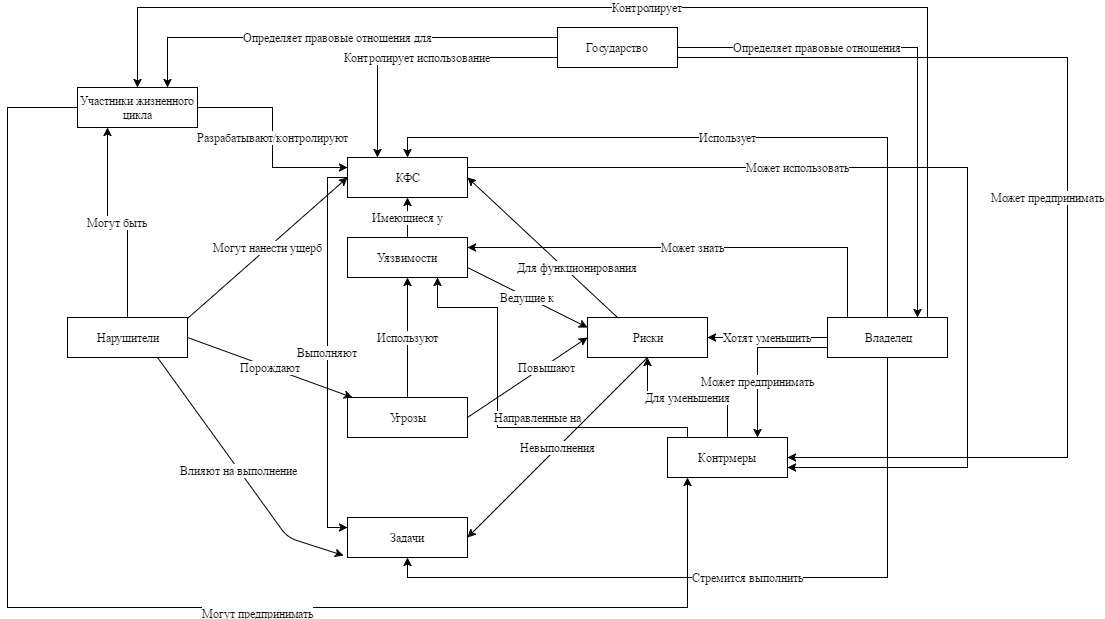
\includegraphics[width=\textwidth]{graphics/термины.png}

    \section{Литература}
    \begin{itemize}
        \item Сурмин Ю. П. Теория систем и системный анализ //К.: МАУП. – 2003. – Т. 364.
        \item Чернышов В. Н., Чернышов А. В. Теория систем и системный анализ. – 2008.
        \item И. И. Викснин, С. В. Маликов, А. И. Чучаев; под ред. А. И. Чучаева. – Москва : Контракт, 2022. – 240 с. Шифр РНБ: 2022-5/6130
        \item Петренко В. И. и др. Анализ рисков нарушения информационной безопасности в роевых робототехнических системах при масштабировании численности агентов //Прикаспийский журнал: управление и высокие технологии. – 2022. – №. 2 (58). – С. 92-109.
        \item Джамалова З. И. и др. Анализ эксплуатационной надежности кибер-физических систем //Вестник Казахской академии транспорта и коммуникаций им. М. Тынышпаева. – 2018. – №. 1. – С. 215-227.
        \item Jia Y. et al. Study on the influence of electromagnetic pulse on UAV communication link //Am. J. Electr. Electron. Eng. – 2019. – Т. 7. – С. 42-48.
        \item Карпова И. П., Карпов В. Э. Агрессия в мире аниматов, или О некоторых механизмах управления агрессивным поведением в групповой робототехнике //Управление большими системами: сборник трудов. – 2018. – №. 76. – С. 173-218.
    \end{itemize}
\end{sloppypar}
\end{document}